\section{Study of a real product}
\label{sec:study-real-product}

% The studied product is an analog regulation function from automotive world
This chapter details a study case of a real \gls{asic} from the automotive field exposed to \gls{esd} during normal operation.
The studied chip performs high-level functions with significant roles inside the vehicle, such as communicating with sensors and performing safety-related duties.
Tests and analysis are focused on one function in particular, the primary voltage regulation function of the device.
In the final application, it is powered directly by the car's battery, and supplies the entire product.
It is also a good opportunity to study the behavior of a complex analog function exposed to electrostatic discharges.
This product was designed at NXP, and complete access to the schematic and layout was made available for this research work.
The product operation, architecture and application are described in section \ref{sec:product-desc}.

% The chip is used in a lighter configuration where a failure could be identified
This chip has a recommended application circuit provided by NXP, and a specification.
They define many requirements to ensure proper operation, such as supply voltage range, current capability, etc.
Among all those requirements is also defined the minimum constraints for external capacitive decoupling and filtering.
Those constraints are not required by the functionality itself, but are needed to ensure good performance against electrical stresses with some decent margin.
In this research study, the amount of external decoupling and filtering has been reduced intentionally.
The objective is to reduce the bill of materials of the complete application and thus to diminish the cost for the equipment manufacturer.
With this lighter configuration, and by running \gls{esd} simulations, it has been possible to discover a functional weakness.
The failure is described in detail in section \ref{sec:failure-case-study}.

\subsection{Product description}
\label{sec:product-desc}

% What kind of product
An automotive \gls{asic} was tested for highlighting a practical case of functional failure.
The studied chip performs several high-level and critical functions for the car vehicle.

% What kind of failure
The failure was discovered while putting the chip in a lowered configuration.
In this configuration, the amount of external devices was reduced.
The goal is to check if the robustness of the chip against \gls{esd}s is impacted.

With the normal configuration, the failure \textbf{never} happens (up to the maximum testing limit).
Failures happen only with the lowered configuration.
As a side note, the lowered configuration is relevant because the \gls{bom} of the system is smaller, and manufacturing costs are reduced.

\begin{figure}[!h]
  \centering
  
\includegraphics[width=0.9\textwidth]{src/3/figures/architecture_system.pdf}
  \caption{Overview of the system architecture}
  \label{fig:system_architecture}
\end{figure}

% Difference of configs
The input used during the tests to inject the \gls{esd} inside the system is the battery supply connection (Fig. \ref{fig:system_architecture}).
The normal configuration uses strong differential and common-mode filtering on this input.
This technique very effectively deviates the stress current into a ground before it even has a chance to reach the chip under test.
In the lowered configuration, only a reduced differential filtering is present on the input.

% What is being tested
Inside the \gls{ic}, the study focuses on the primary supply function (Fig. \ref{fig:monitored_function}).
This function is the first to start when the chip is powered-on.
It powers many blocks, especially sensitive digital cells and low-voltage analog functions.

% Why testing this function
There are two motivations for testing this particular function.
One of its input (battery input) is an external pin and is also exposed as the system level.
This pin can very likely be exposed to electrostatic discharges during real operation.
Then, one of its output is also exposed externally, because the function requires a large capacitor for stabilisation that cannot be integrated on silicon.
This pin is a very convenient monitoring point during tests.

%TODO: Increase font size
\begin{figure}[!h]
  \centering
  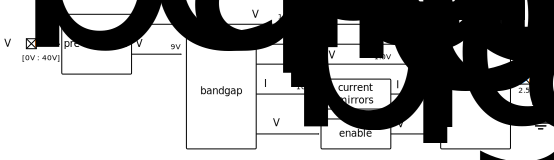
\includegraphics[width=0.9\textwidth]{src/3/figures/monitored_function.pdf}
  \caption{Architecture of the primary supply}
  \label{fig:monitored_function}
\end{figure}


\subsubsection{Integrated supply function description}
\label{sec:supply-desc}

% Main task
The main function of the regulation function is to down-convert a battery voltage to a 2.5V regulated supply.
Several blocks are involved for processing the battery supply.
The overall architecture is given in fig. \ref{fig:monitored_function}).

%TODO: Uniform net names
% First block
First, a pre-regulator clamps the battery input (V\textsubscript{batt}) that can reach up to 40V and down to 9V.
This is done to protect more sensitive circuitry connected downstream.
This clamped voltage is accessible on output V\textsubscript{clamp9}.
V\textsubscript{clamp9} has low current capability and is used for low-power functions.
A second output V\textsubscript{pwr} provides a 12V clamped output with a large current capability.

% Second block
A bandgap reference is connected downstream.
It is powered with V\textsubscript{clamp9}.
Once properly started after a certain delay, the bandgap generates a 1.0 V voltage reference on V\textsubscript{ref1p0}.
This reference is stable accross a wide range of temperature, process variation and process mismatchs.
The bandgap also outputs a 10uA current reference on I\textsubscript{ref10u}, and a flag V\textsubscript{bgok} to signal it is ready for operation.

% Third major block
Finally, the \gls{ldo} regulator generates a stable 2.5V supply voltage on V\textsubscript{2p5}.
This output can deliver up to 20mA.
V\textsubscript{2p5} is used further in the system to power digital gates.

% Detail nets connections
The regulator relies on multiple signals generated in the upstream blocks for operation.
The most critical nets are the 1.0V reference V\textsubscript{ref1p0} from the bandgap, and the ramp-up signal V\textsubscript{ramp-up}.
Circuit analysis shows that both nets can directly affect the output voltage.
A variation on the reference voltage is immediately copied on the output.
The ramp-up signal controls the soft-start of the regulator, that can directly change the output value.
Other nets provide bias to the regulator, and their impact on the output is more limited.

% Talk about external devices
V\textsubscript{2p5} requires externally a 100nF decoupling capacitor to absorb peak currents and achieve stability.

% What are the minor blocks doing
The \textit{current mirrors} provide copied current values from the bandgap, while offering much larger output impedance.
The \textit{enable} block mostly checks and waits for the bandgap to be properly started.
It then triggers a startup ramp-up sequence on the regulator.

\subsection{Functional failure study}
\label{sec:failure-case-study}

% How does it happen
The failure can be induced by injecting a negative-voltage \gls{esd} discharge on the battery input pin (Fig. \ref{XX}).
The \gls{ESD} is superimposed on the DC battery voltage, when the product is in operation.
This input is a realistic entry point for an \gls{esd}.
Indeed, it is connected directly to the integrated circuit, but it is exposed at the system level.
The battery is connected to this input by a cable, which is a frequent entry point for \gls{esd} (Source ?).

TODO: SCHEMA injection setup

% What is the result
The failure can be observed on the regulated 2.5V supplies, and in general on the entire system's behavior.
With a sufficiently large negative stress, the regulated output is disturbed and goes into soft-start (Fig. \ref{XX}).
A soft-start is a special sequence, normally happening when the device is first powered-on.
During this sequence, the supply voltage slowly rises from 0V to its nominal value, to avoid overshoots that could damage sensitive blocks.
Soft-starts can last from tens to hundreds of microseconds (source ?).
As a consequence the entire integrated functions are not available during the soft-start.
Some functions can be disturbed for much longer if they also need to follow their own startup sequences.

TODO: MEASUREMENT FAILURE OUTPUT

% Talk about the scale factor
To summarize, a negative stress of a hundred nanoseconds induces here a supply restart of tens of microseconds.
Parts of the system can be disturbed for much longer.
There is a scale factor of at least 100 between the stress width and the regulation function.
In this study, we try to explain how an \gls{esd} can generate such a scale factor.

\subsubsection{Study through simulation}

% Is the simulation accurate
To understand the failure mechanism, top-level simulations are first ran to see if the global failure can be reproduced.
A simulation setup is built to match closely the real circuit.
The \gls{tlp} model (described in section \ref{sec:tlp-modeling}) is also employed.
The external input and output voltage waveforms are compared in Fig. \ref{fig:wvf-vboost} (input) and Fig. \ref{fig:wvf-v2p5} (output).
Both curves correlate well, and the regulator restart is correctly reproduced in simulation.
These results tend to indicate that the simulations can be trusted for this study case.

% TODO: MEASUREMENT vs SIMULATION
\begin{figure}[!htbp]
  \centering
  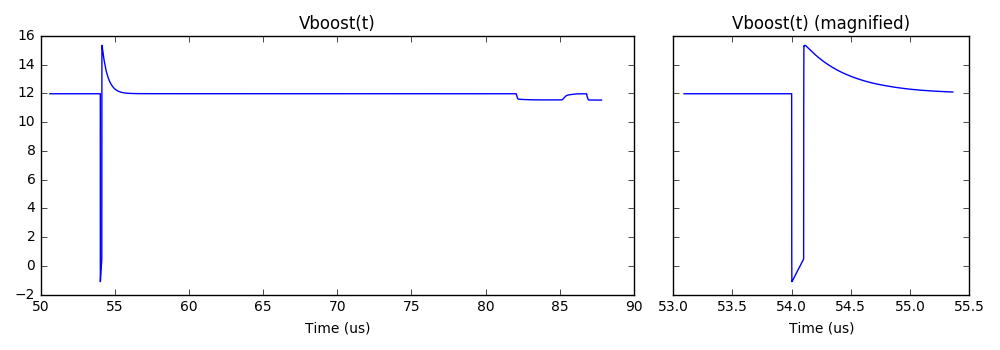
\includegraphics[width=0.9\textwidth]{src/3/figures/vboost.png}
  \caption{Waveform of the vboost input pin}
  \label{fig:wvf-vboost}
\end{figure}

\begin{figure}[!htbp]
  \centering
  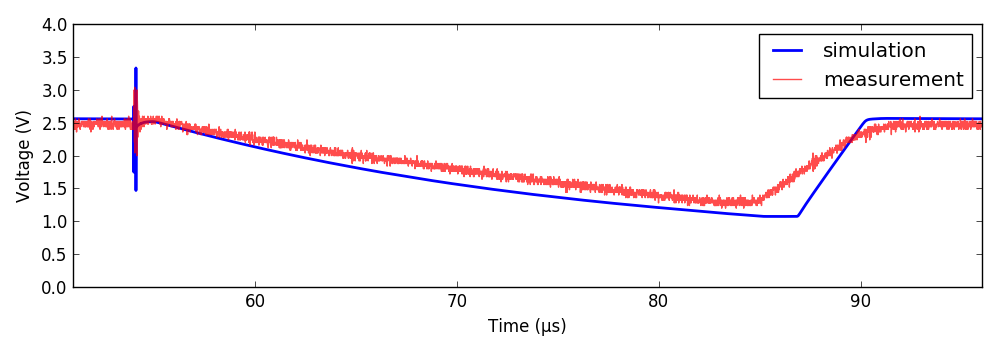
\includegraphics[width=0.9\textwidth]{src/3/figures/v2p5.png}
  \caption{Waveform of the v2p5 output pin}
  \label{fig:wvf-v2p5}
\end{figure}

% Make the investigation
The investigation process is now conducted.
The injected stress is a rectangular pulse of -100V amplitude and 100ns width.
The main output of the first block (the pre-regulator) is observed in simulation (Fig. \ref{fig:wvf-vclamp9}).
At 54 \textmugreek{}s, its \textit{vclamp9} output voltage is clearly disturbed by the negative stress.
The net reaches as low as 0V for a brief amount of time.
Overall, the net is disturbed for 750 ns.

% Next net, bandgap input
In turn, this net powers the bandgap reference.
Thus, it can be expected that the bandgap is going to be disturbed as well.
The observation of the 1.0V bandgap reference \textit{vref1p0} confirms it (Fig. \ref{fig:wvf-v1p0}).
The reference drops down to 0.25V, and is disturbed for about 3 \textmugreek{}s.

\begin{figure}[!htbp]
  \centering
  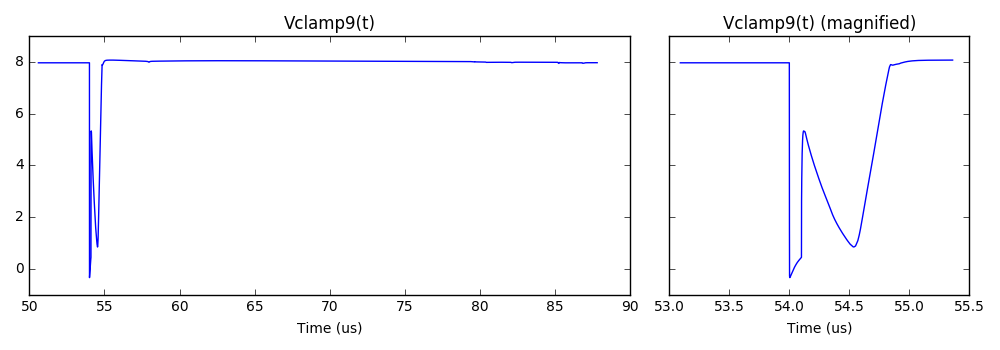
\includegraphics[width=0.9\textwidth]{src/3/figures/vclamp9.png}
  \caption{Waveform of the vclamp9 internal net}
  \label{fig:wvf-vclamp9}
\end{figure}

\begin{figure}[!htbp]
  \centering
  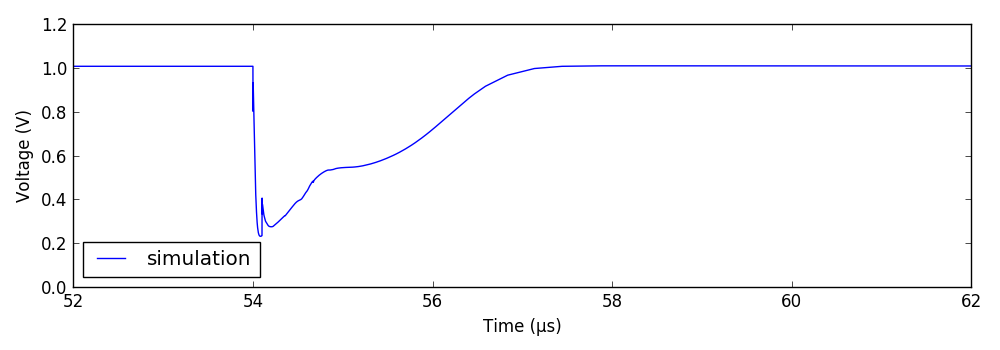
\includegraphics[width=0.9\textwidth]{src/3/figures/v1p0.png}
  \caption{Waveform of the vref1p0 internal net}
  \label{fig:wvf-v1p0}
\end{figure}

%TODO: Most likely, this needs to be reviewed later and detailed more.
% Final net
Finally, this bandgap reference is used by the regulator to generate the 2.5 V external supply output.
Net \textit{v2p5} drops below 1.5V, and is disturbed for more than 30 \textmugreek{}s.
Clearly, the scale factor is well reproduced in the simulation.

% Preliminary conclusion with scale factor
In the first block (pre-regulator), the disturbance width increased from 100 ns to 750 ns.
In the second block (bandgap), it increased from 750 ns to 3 \textmugreek{}s.
In the third block (regulator), it reached 30 \textmugreek{}s.
Each time, there is an aggravation of the failure.

%TODO: Make full schematic analysis ?

% Talk about failure in cascade
To conclude, it appears there is a failure in cascade of the regulation function.
When the disturbance propagates through a block, it is amplified and becomes more severe.
Ultimately, a function that takes a lot of time to recover (soft-start) is hit, causing a full system restart.

The next part of this research work is focused on acquiring measurement data on silicon, to confirm the simulations.
Also, this study case remains simple to understand, but fixing the issue is difficult.
It must be ensured that a circuit correction for \gls{esd} does not affect normal operation.
In practice this can be difficult, because both can have opposite requirements.
There are also many situations where the failure cause is not so obvious, and calls for advanced investigation methods.

For these purposes a testchip is designed in next section \ref{sec:test-vehicle-desc}.
Modeling methods are explored in section \ref{sec:bottom-up-modeling} as a way to understand better these issues.

